% !TEX encoding = UTF-8 Unicode
%%%%%%%%%%%%%%%%%%%%%%%%%%%%%%%%%%%%%%%%%%%%%%%%%%%%%%%%%%%%%%%%%%%%%%%%%%%%%%%%
% Caelum Post-Flight Offline Dashboard Analysis — Unified Engineering Manuscript
% ASME conference style draft focused on the MATLAB post-flight analysis stack.
%%%%%%%%%%%%%%%%%%%%%%%%%%%%%%%%%%%%%%%%%%%%%%%%%%%%%%%%%%%%%%%%%%%%%%%%%%%%%%%%

\providecommand\DocumentMetadata[1]{}
\DocumentMetadata{
  lang        = eng-US,
  pdfstandard = A-3u,
  pdfversion  = 1.7
}

\documentclass[colorlinks,upint,subscriptcorrection,varvw,hyphenate,balance]{asmeconf}

\hypersetup{%
  pdfauthor   = {David Richardson},
  pdftitle    = {Caelum: A MATLAB Post-Flight Offline Dashboard for Replay-Based Estimation, Event Detection, and Flight-Test Review},
  pdfkeywords = {MATLAB, post-flight analysis, telemetry, dashboard, EKF, quaternion, replay, flight test, validation},
  pdfsubject  = {Unified engineering manuscript for the Caelum MATLAB post-flight offline dashboard analysis project}
}

\allowdisplaybreaks
\emergencystretch=1em

\usepackage[T1]{fontenc}
\usepackage[utf8]{inputenc}
\usepackage{textcomp}
\usepackage{microtype}
\usepackage{amsmath,mathtools}
\usepackage{siunitx}
\usepackage{booktabs}
\usepackage{graphicx}
\graphicspath{{figures/}{./}}
\usepackage{tabularx}
\usepackage{array}
\usepackage{makecell}
\usepackage{adjustbox}
\usepackage{ragged2e}
\usepackage{multirow}
\usepackage{enumitem}
\usepackage{tikz}
\usepackage{pgfplots}
\pgfplotsset{compat=1.18}
\usetikzlibrary{arrows.meta,positioning,shapes.geometric,calc,fit,backgrounds}

\newcolumntype{Y}{>{\RaggedRight\arraybackslash}X}
\newcolumntype{C}{>{\Centering\arraybackslash}X}
\newcommand{\code}[1]{\texttt{\allowbreak#1}}
\newcommand{\pkg}{\code{+caelum}}
\newcommand{\TT}{\code{timetable}}
\newcommand{\dt}{\Delta t}
\newcommand{\R}{\mathbf{R}}
\newcommand{\q}{\mathbf{q}}
\newcommand{\x}{\mathbf{x}}
\newcommand{\uvec}{\mathbf{u}}
\newcommand{\z}{\mathbf{z}}
\newcommand{\Pcov}{\mathbf{P}}
\newcommand{\Qcov}{\mathbf{Q}}
\newcommand{\Rcov}{\mathbf{R}}
\newcommand{\gvec}{\mathbf{g}}
\newcommand{\avec}{\mathbf{a}}
\newcommand{\vvec}{\mathbf{v}}
\newcommand{\pvec}{\mathbf{p}}
\newcommand{\wvec}{\boldsymbol{\omega}}
\newcommand{\verticalDashboardFigure}{figures/caelum_vertical_dashboard_v1.png}

\ConfName{Proceedings of the ASME 2026\linebreak International Design Engineering Technical Conferences and Computers and Information in Engineering Conference}
\ConfAcronym{IDETC/CIE2026}
\ConfDate{August 23--26, 2026}
\ConfCity{Houston, TX}
\PaperNo{DETC2026-XXXX}

\title{CAELUM: A MATLAB POST-FLIGHT OFFLINE DASHBOARD FOR REPLAY-BASED ESTIMATION, EVENT DETECTION, AND FLIGHT-TEST ENGINEERING REVIEW}

\SetAuthors{%
  David Richardson\affil{1}\CorrespondingAuthor{davirich@umich.edu}
}
\SetAffiliation{1}{University of Michigan--Dearborn, Dearborn, MI, USA}

\keywords{MATLAB, Post-Flight Analysis, Telemetry Replay, Extended Kalman Filter, Quaternion Attitude, Dashboard, Flight-Test Validation}

\begin{document}
\maketitle

\begin{abstract}
Caelum is a MATLAB post-flight analysis project that converts flight logs into a reproducible offline engineering dashboard. The project is organized around a replay doctrine: imported telemetry is aligned to a documented schema, cleaned, enriched with attitude and estimator fields, processed by vertical and three-dimensional estimation routines, annotated with detected events, summarized into tabular metrics, and visualized through overview, dashboard, three-dimensional, firmware-replay, and Monte Carlo views. The implementation is represented by a MATLAB package namespace, \pkg{}, containing import utilities, schema alignment, event detection, quaternion mathematics, vertical and 3D extended Kalman filter (EKF) routines, firmware log support, summary/export tools, and plotting functions. The supplied dashboard screenshots show two important review modes: a dense vertical-replay diagnostic dashboard and an integrated V3 dashboard containing GPS fusion, 3D trajectory, wind estimation, and event timing. This manuscript provides a unified explanation of the project and its design discussions in an ASME conference style. The emphasis is rigorous engineering traceability: each plotted dashboard quantity must be attributable to an import contract, a state-estimation replay, an explicit derived metric, or a validation artifact. The resulting workflow supports post-flight diagnosis, estimator comparison, release validation, and archival reporting without relying on manual plotting or undocumented analyst judgment.
\end{abstract}

\begin{nomenclature}
\EntryHeading{Time and replay}
\entry{$t_k$}{Timestamp at sample $k$}
\entry{$\dt_k$}{Elapsed time between samples $k-1$ and $k$}
\entry{\TT}{MATLAB time-indexed table used for aligned telemetry}
\entry{\code{log}}{Imported flight-log table, timetable, or structure}
\entry{\code{cfg}}{Configuration structure returned by \code{defaultConfig}}

\EntryHeading{State estimation}
\entry{$\x$}{Estimator state vector}
\entry{$\Pcov$}{State covariance matrix}
\entry{$\Qcov$}{Process-noise covariance}
\entry{$\Rcov$}{Measurement-noise covariance}
\entry{$\z$}{Measurement vector}
\entry{$\pvec$}{Position vector}
\entry{$\vvec$}{Velocity vector}
\entry{$h$}{Altitude or vertical position}
\entry{$b_a$}{Accelerometer bias term}

\EntryHeading{Attitude and kinematics}
\entry{$\q=[q_w,q_x,q_y,q_z]^T$}{Unit quaternion attitude representation}
\entry{$\phi,\theta,\psi$}{Roll, pitch, and yaw angles}
\entry{$\R(\q)$}{Rotation matrix formed from quaternion $\q$}
\entry{$\wvec$}{Angular-rate vector}
\entry{$\gvec_b$}{Gravity vector expressed in body coordinates}

\EntryHeading{Acronyms}
\entry{EKF}{Extended Kalman filter}
\entry{GPS}{Global Positioning System}
\entry{IMU}{Inertial measurement unit}
\entry{SD}{Secure Digital storage}
\entry{KPI}{Key performance indicator}
\entry{CSV}{Comma-separated values}
\end{nomenclature}

%==============================================================================
\section{INTRODUCTION}
%==============================================================================

The Caelum project addresses a common problem in flight-test engineering: flight logs are rich enough to explain vehicle behavior, but only after they are reconstructed into a coherent analysis product. Raw logs rarely arrive in a form suitable for immediate interpretation. They may contain mixed field names, missing values, variable sampling intervals, estimator outputs from different algorithm generations, firmware-specific SD-card schemas, and truth or simulation fields used during validation. A rigorous post-flight dashboard must therefore perform disciplined reconstruction before it performs visualization. MATLAB tables and timetables provide a natural substrate for this type of time-indexed engineering analysis \cite{matlab_timetable}.

The MATLAB codebase is structured as a package namespace, \pkg{}, with entry points such as \code{run\_caelum\_example.m}, \code{validate\_caelum\_release.m}, and \code{validate\_vertical\_replay\_stack.m}. The package-level functions include log import, robust schema alignment, cleaning, event detection, vertical and 3D EKF replay, quaternion propagation, wind estimation, dashboard plotting, summary export, figure export, firmware replay, and Monte Carlo validation. The dashboard is consequently not a single plot; it is the presentation layer of a larger offline analysis stack.

This manuscript unifies the project intent and engineering discussions into a single ASME-style technical document. The central claim is that Caelum should be understood as a deterministic post-flight replay system: given the same log package and configuration, it should produce the same cleaned telemetry, estimator histories, detected events, summary tables, and figures.

\subsection{Contributions}
The project makes four engineering contributions:
\begin{enumerate}[leftmargin=*,nosep]
\item a MATLAB package architecture for post-flight telemetry import, schema alignment, replay, and visualization;
\item a vertical replay stack connecting imported telemetry to a vertical EKF, firmware-compatible estimator path, and validation contract;
\item a 3D extension path incorporating quaternion attitude handling, GPS update logic, and three-dimensional overview plots; and
\item a release-validation doctrine connecting examples, synthetic truth-aware logs, Monte Carlo validation, exported figures, and dashboard outputs.
\end{enumerate}

%==============================================================================
\section{PROJECT SCOPE AND ARTIFACTS}
%==============================================================================

\subsection{In-Scope Engineering Functions}
The manuscript covers the MATLAB offline analysis system represented by the following functional groups:
\begin{itemize}[leftmargin=*]
\item \textbf{Execution and validation:} \code{run\_caelum\_example}, \code{validate\_caelum\_release}, and \code{validate\_vertical\_replay\_stack}.
\item \textbf{Import and schema control:} \code{importLog}, \code{importLogRobust}, \code{alignImportedSchema}, \code{getFirmwareSdlogSchema}, and \code{getVerticalReplayFieldContract}.
\item \textbf{Cleaning and enrichment:} \code{cleanLog}, \code{attachPhase1AttitudeFields}, and \code{defaultConfig}.
\item \textbf{Estimation replay:} \code{runVerticalEKF}, \code{predictVerticalEKF}, \code{updateVerticalEKFBaro}, \code{run3DEKF}, \code{predict3DEKF}, and \code{update3DEKFGPS}.
\item \textbf{Attitude mathematics:} \code{normalizeQuaternion}, \code{propagateQuaternion}, \code{quaternionToRotationMatrix}, \code{quaternionToEulerZYX}, \code{gravityBodyFromQuaternion}, and \code{localExtractQuaternion}.
\item \textbf{Analysis products:} \code{analyzeLog}, \code{detectEvents}, \code{estimateWind}, \code{summarizeLog}, \code{makeSummaryTable}, \code{exportSummary}, and \code{exportFigures}.
\item \textbf{Visualization and validation views:} \code{plotDashboard}, \code{plotOverview}, \code{plotOverview3D}, \code{plotMonteCarloSummary}, \code{runMonteCarloValidation}, and truth-aware log generators.
\item \textbf{Firmware-facing replay:} \code{runRealtimeOnboard} and \code{runFirmwareVerticalEstimator}.
\end{itemize}

\subsection{Out-of-Scope Topics}
This manuscript does not claim flight-critical certification, real-time autopilot implementation, airframe structural validation, or a complete aerodynamic model. The focus is post-flight reconstruction and analysis of telemetry already recorded by the vehicle, firmware, or simulation environment.

\subsection{Document Position}
The LaTeX style follows the provided ASME conference manuscript reference. The technical subject is different: this paper explains the MATLAB post-flight dashboard analysis project rather than the prior sonar-camera FPGA system.

%==============================================================================
\section{ENGINEERING DOCTRINE}
%==============================================================================

\subsection{Replay Before Interpretation}
The dashboard is meaningful only after the flight has been replayed into a coherent analysis state. Raw columns are not plotted directly unless they have passed through import, schema alignment, cleaning, and unit/field validation. This rule prevents visually polished plots from masking inconsistent log semantics.

\subsection{Configuration as an Analysis Input}
The function \code{defaultConfig} should be treated as part of the experiment definition. Noise assumptions, thresholds, plotting defaults, event limits, and estimator options are not incidental constants; they define the analysis context and must be reproducible.

\subsection{Schema Contracts Over Guesswork}
The presence of \code{alignImportedSchema}, \code{getFirmwareSdlogSchema}, and \code{getVerticalReplayFieldContract} indicates a project-level decision: imported logs must satisfy field contracts. This is especially important when the same analysis stack is expected to operate on synthetic logs, MATLAB-generated truth-aware logs, firmware SD logs, and possibly user-supplied CSV exports.

\subsection{Plots Are Derived Evidence}
The dashboard, overview plots, 3D plots, and Monte Carlo summaries are presentation artifacts. Their authority comes from the processing chain beneath them: \code{analyzeLog}, estimator replay, event detection, and summary generation.

%==============================================================================
\section{ARCHITECTURE OF THE OFFLINE ANALYSIS STACK}
%==============================================================================

Figure~\ref{fig:pipeline} summarizes the Caelum workflow inferred from the package organization.

\begin{figure*}[t]
\centering
\begin{adjustbox}{max width=0.98\textwidth}
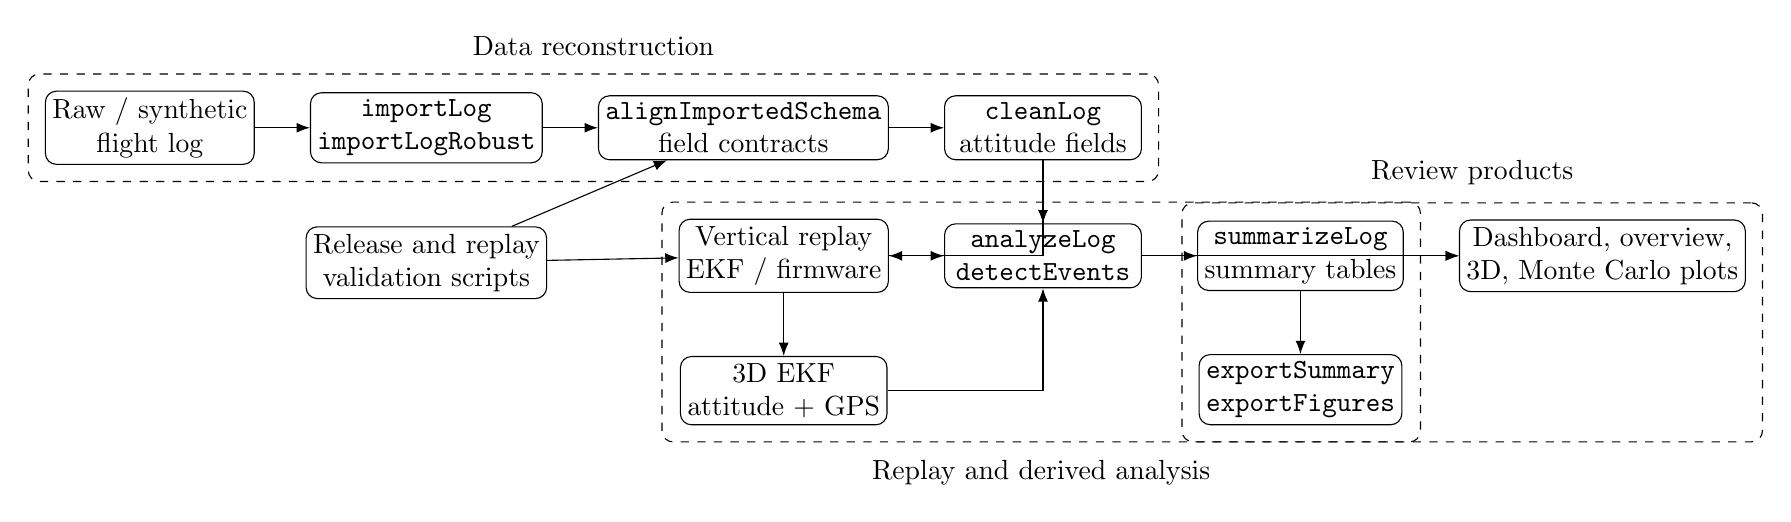
\begin{tikzpicture}[
    node distance=8mm and 7mm,
    blk/.style={draw, rounded corners, align=center, minimum width=25mm, minimum height=8mm, inner sep=2.5pt},
    grp/.style={draw, dashed, rounded corners, inner sep=6pt},
    >=Latex
]
\node[blk] (raw) {Raw / synthetic\\flight log};
\node[blk, right=of raw] (import) {\code{importLog}\\\code{importLogRobust}};
\node[blk, right=of import] (schema) {\code{alignImportedSchema}\\field contracts};
\node[blk, right=of schema] (clean) {\code{cleanLog}\\attitude fields};
\node[blk, below=of clean] (analysis) {\code{analyzeLog}\\\code{detectEvents}};
\node[blk, left=of analysis] (vertical) {Vertical replay\\EKF / firmware};
\node[blk, below=of vertical] (threeD) {3D EKF\\attitude + GPS};
\node[blk, right=of analysis] (summary) {\code{summarizeLog}\\summary tables};
\node[blk, right=of summary] (plots) {Dashboard, overview,\\3D, Monte Carlo plots};
\node[blk, below=of summary] (export) {\code{exportSummary}\\\code{exportFigures}};
\node[blk, below=of import] (valid) {Release and replay\\validation scripts};
\draw[->] (raw) -- (import);
\draw[->] (import) -- (schema);
\draw[->] (schema) -- (clean);
\draw[->] (clean) -- (analysis);
\draw[->] (clean) |- (vertical);
\draw[->] (vertical) -- (threeD);
\draw[->] (vertical) -- (analysis);
\draw[->] (threeD) -| (analysis);
\draw[->] (analysis) -- (summary);
\draw[->] (summary) -- (plots);
\draw[->] (summary) -- (export);
\draw[->] (analysis) -- (plots);
\draw[->] (valid) -- (schema);
\draw[->] (valid) -- (vertical);
\node[grp, fit=(raw)(import)(schema)(clean)] (g1) {};
\node[above=1mm of g1.north] {Data reconstruction};
\node[grp, fit=(vertical)(threeD)(analysis)(summary)] (g2) {};
\node[below=1mm of g2.south] {Replay and derived analysis};
\node[grp, fit=(plots)(export)] (g3) {};
\node[above=1mm of g3.north] {Review products};
\end{tikzpicture}
\end{adjustbox}
\caption{Project-level Caelum analysis pipeline. The dashboard is downstream of schema alignment, cleaning, replay-based estimation, event detection, and summary generation.}
\label{fig:pipeline}
\end{figure*}

\subsection{Primary Execution Path}
A typical user-facing workflow begins with \code{run\_caelum\_example.m}. The script should be understood as a reproducible demonstration path: generate or load a log, import it, run the analysis stack, produce dashboard figures, and export summaries. Such an example is important because it provides a stable entry point for users and a regression target for release validation.

\subsection{Release Validation Path}
\code{validate\_caelum\_release.m} is the release-level guardrail. It should exercise representative data paths and assert that the package can still import, clean, replay, summarize, plot, and export after code changes. \code{validate\_vertical\_replay\_stack.m} serves a narrower role: it protects the vertical estimator pathway and its field contract.

\subsection{Package Boundary}
The \pkg{} namespace provides a clean boundary between reusable analysis functions and top-level scripts. This division is valuable because top-level scripts may choose a scenario, but package functions define the behavior that must remain stable across scenarios.

%==============================================================================
\section{DATA INGEST, SCHEMA ALIGNMENT, AND CLEANING}
%==============================================================================

\subsection{Import Strategy}
The coexistence of \code{importLog} and \code{importLogRobust} suggests two import levels: a standard loader and a more defensive loader for logs with missing, reordered, or variant fields. A rigorous offline dashboard should prefer the robust path for user-facing workflows and reserve the simpler path for controlled examples or tests.

\subsection{Schema Alignment}
The function \code{alignImportedSchema} is central to cross-log repeatability. Its role is to map variant source fields into the canonical Caelum field set expected by replay and plotting functions. Without this stage, every downstream routine would need to know every historical firmware or simulator column name.

\subsection{Firmware SD Log Contract}
\code{getFirmwareSdlogSchema} records the expected firmware SD-card log structure. This turns firmware import from an informal convention into a reviewable interface. When firmware fields change, the schema definition is the natural location to update and validate the contract.

\subsection{Vertical Replay Field Contract}
\code{getVerticalReplayFieldContract} identifies which fields the vertical replay stack requires, which are optional, and which are produced downstream. This makes the vertical estimator auditable and reduces the probability that a plot silently degrades because a needed input field was absent.

\begin{table*}[t]
\caption{Representative Caelum data contracts}
\centering
\begin{tabularx}{\textwidth}{l Y Y}
\toprule
Contract artifact & Engineering role & Failure mode prevented \\
\midrule
\code{defaultConfig} & Defines estimator, plotting, threshold, and analysis parameters & Hidden tuning drift between analyses \\
\code{importLogRobust} & Handles less regular input logs and prepares them for schema alignment & Fragile import behavior on real logs \\
\code{alignImportedSchema} & Maps imported fields to canonical Caelum names & Downstream functions depending on source-specific column names \\
\code{getFirmwareSdlogSchema} & Documents firmware SD log fields and expected semantics & Ambiguous firmware-to-MATLAB integration \\
\code{getVerticalReplayFieldContract} & Declares required vertical replay inputs and outputs & Estimator replay with incomplete telemetry \\
\code{cleanLog} & Removes or repairs invalid samples and prepares analysis-ready data & Dashboard plots driven by malformed records \\
\bottomrule
\end{tabularx}
\label{tab:contracts}
\end{table*}

\subsection{Cleaning and Enrichment}
\code{cleanLog} is the appropriate location for missing-data handling, sample rejection, type normalization, and monotonicity checks. \code{attachPhase1AttitudeFields} enriches the log with attitude fields used by later plots and estimators. This split is valuable: cleaning establishes data validity, while enrichment adds derived state needed for interpretation.

%==============================================================================
\section{REPLAY-BASED ESTIMATION}
%==============================================================================

\subsection{Vertical EKF Stack}
The vertical replay stack is represented by \code{initializeVerticalEKFState}, \code{runVerticalEKF}, \code{predictVerticalEKF}, and \code{updateVerticalEKFBaro}. A common vertical state form is
\begin{equation}
\x_v =
\begin{bmatrix}
h & v_z & b_a
\end{bmatrix}^T,
\label{eq:vertical_state}
\end{equation}
where $h$ is vertical position, $v_z$ is vertical velocity, and $b_a$ is accelerometer bias. A representative discrete prediction model is
\begin{equation}
\begin{aligned}
h_{k+1} &= h_k + v_{z,k}\dt_k + \frac{1}{2}(a_{z,k}-b_{a,k})\dt_k^2,\\
v_{z,k+1} &= v_{z,k} + (a_{z,k}-b_{a,k})\dt_k,\\
b_{a,k+1} &= b_{a,k}.
\end{aligned}
\label{eq:vertical_predict}
\end{equation}
The barometric update in \code{updateVerticalEKFBaro} can be interpreted as a measurement correction of the altitude component,
\begin{equation}
\z_k = h_k + \nu_k,
\qquad
\nu_k \sim \mathcal{N}(0,R_h).
\label{eq:baro_update}
\end{equation}

\subsection{General EKF Form}
Both the vertical and 3D estimators follow the standard EKF structure \cite{welch}:
\begin{equation}
\hat{\x}_{k|k-1}=f(\hat{\x}_{k-1|k-1},\uvec_k,\dt_k),
\label{eq:ekf_predict_state}
\end{equation}
\begin{equation}
\Pcov_{k|k-1}=\mathbf{F}_k\Pcov_{k-1|k-1}\mathbf{F}_k^T+\Qcov_k,
\label{eq:ekf_predict_cov}
\end{equation}
\begin{equation}
\mathbf{K}_k=\Pcov_{k|k-1}\mathbf{H}_k^T
\left(\mathbf{H}_k\Pcov_{k|k-1}\mathbf{H}_k^T+\Rcov_k\right)^{-1},
\label{eq:kalman_gain}
\end{equation}
\begin{equation}
\hat{\x}_{k|k}=\hat{\x}_{k|k-1}+\mathbf{K}_k
\left(\z_k-h(\hat{\x}_{k|k-1})\right).
\label{eq:ekf_update}
\end{equation}
The dashboard should never display estimator states without making clear whether they are imported firmware estimates, MATLAB replay estimates, or truth-aware simulation quantities.

\subsection{Three-Dimensional EKF Stack}
The 3D path is represented by \code{initialize3DEKFState}, \code{run3DEKF}, \code{predict3DEKF}, \code{update3DEKFGPS}, \code{localResolve3DConfig}, and \code{localExtractGPSMeasurement}. This stack extends the vertical analysis to position, velocity, attitude-informed gravity compensation, and GPS correction. A representative 3D navigation state is
\begin{equation}
\x_3 =
\begin{bmatrix}
\pvec^T & \vvec^T & \q^T & \mathbf{b}_a^T & \mathbf{b}_g^T
\end{bmatrix}^T.
\label{eq:state_3d}
\end{equation}
The exact implemented state may differ, but the manuscript-level contract is that \code{run3DEKF} produces a replay history whose provenance is separate from raw log fields and whose configuration is resolved explicitly.

\subsection{Firmware-Compatible Estimation}
\code{runRealtimeOnboard} and \code{runFirmwareVerticalEstimator} connect the offline dashboard to onboard-style estimation behavior. Their presence is important because the dashboard can compare MATLAB replay results against firmware-compatible logic rather than only against an idealized offline estimator.

%==============================================================================
\section{ATTITUDE AND QUATERNION PROCESSING}
%==============================================================================

\subsection{Quaternion Normalization}
Attitude replay depends on valid unit quaternions. Quaternion methods are standard in strapdown navigation because they provide a compact rotation representation and avoid the singularities associated with Euler-only state propagation \cite{titterton,kuipers}. The function \code{normalizeQuaternion} should enforce
\begin{equation}
\q_{\mathrm{unit}} = \frac{\q}{\lVert\q\rVert_2},
\label{eq:quat_norm}
\end{equation}
with appropriate handling for degenerate inputs. This prevents attitude plots and gravity compensation from drifting because of numerical scale error.

\subsection{Quaternion Propagation}
\code{propagateQuaternion} advances attitude using angular-rate measurements. A standard continuous relation is
\begin{equation}
\dot{\q} = \frac{1}{2}\Omega(\wvec)\q,
\label{eq:quat_prop}
\end{equation}
where $\Omega(\wvec)$ is the quaternion rate matrix formed from body angular rates. The propagated quaternion should be renormalized to preserve unit length over replay.

\subsection{Rotation Matrix and Euler Conversion}
\code{quaternionToRotationMatrix} and \code{quaternionToEulerZYX} serve different audiences. Rotation matrices are appropriate for vector transformations and estimator math, while ZYX Euler angles are appropriate for dashboard display as yaw, pitch, and roll. The display conversion must not replace quaternion arithmetic inside the estimator.

\subsection{Gravity in Body Coordinates}
\code{gravityBodyFromQuaternion} expresses gravity in the vehicle body frame,
\begin{equation}
\gvec_b = \R(\q)^T
\begin{bmatrix}
0 & 0 & g
\end{bmatrix}^T,
\label{eq:gravity_body}
\end{equation}
or the equivalent convention used by the implementation. This quantity is central to acceleration interpretation and to separating inertial acceleration from gravity in replay analysis.

%==============================================================================
\section{EVENT DETECTION, WIND ESTIMATION, AND SUMMARIZATION}
%==============================================================================

\subsection{Event Detection}
\code{detectEvents} converts telemetry into reviewable occurrences. Events may include launch, burnout, apogee, landing, estimator anomalies, excessive residuals, high-current intervals, loss of GPS-like measurements, aggressive attitude excursions, or firmware status changes. The screenshots show these events used both as vertical dashed markers on time-series panels and as event-timing bars in the integrated dashboard. The important property is not the particular event list, but that events are algorithmically detected and timestamped rather than manually inferred from plots.

\subsection{Wind Estimation}
\code{estimateWind} indicates that Caelum includes derived environmental interpretation. In a simplified kinematic form, wind can be estimated from the difference between inertial ground velocity and air-relative velocity,
\begin{equation}
\mathbf{w}_{\mathrm{wind}} =
\vvec_{\mathrm{ground}} - \vvec_{\mathrm{air}}.
\label{eq:wind}
\end{equation}
If direct airspeed is unavailable, the implemented routine may instead estimate wind from trajectory residuals or synthetic truth-aware fields. In all cases, the dashboard should label wind estimates as derived quantities with assumptions.

\subsection{Summary Products}
\code{summarizeLog} and \code{makeSummaryTable} convert replay histories and detected events into compact engineering products. \code{exportSummary} and \code{exportFigures} then make those products portable for reports, design reviews, and release notes.

\begin{table}[t]
\caption{Representative dashboard summary metrics}
\centering
\begin{tabularx}{\columnwidth}{l Y}
\toprule
Metric class & Example interpretation \\
\midrule
Duration and sample count & Confirms the analyzed flight window and log completeness \\
Altitude extrema & Supports vertical performance and envelope review \\
Estimator residuals & Identifies disagreement between prediction and measurement updates \\
Attitude extrema & Flags aggressive or abnormal vehicle orientation \\
Event counts & Summarizes detected anomalies and phase transitions \\
Energy or current statistics & Connects mission behavior to electrical loading \\
Wind estimate statistics & Supports environmental interpretation of flight behavior \\
\bottomrule
\end{tabularx}
\label{tab:summary_metrics}
\end{table}

%==============================================================================
\section{DASHBOARD AND VISUALIZATION LAYERS}
%==============================================================================

\subsection{Dashboard Role}
\code{plotDashboard} is the integrated review surface. Its purpose is to present synchronized time histories, estimator outputs, events, and summary statistics in a form that supports engineering diagnosis. The dashboard should emphasize traceability: a plotted line should correspond to a named raw field, cleaned field, replay state, event annotation, or summary metric.

\subsection{Overview and 3D Views}
\code{plotOverview} provides a conventional two-dimensional overview of the flight log and derived quantities. \code{plotOverview3D} extends this to spatial interpretation, which is valuable when estimator behavior depends on geometry, trajectory, or GPS correction.

\subsection{Monte Carlo Summary}
\code{runMonteCarloValidation} and \code{plotMonteCarloSummary} support statistical validation. This is important because a single flight or synthetic log can pass while an estimator remains fragile across noise seeds, initial conditions, or trajectory variations. Monte Carlo output should report distributions, not only pass/fail status.

\subsection{Vertical-Replay Diagnostic Dashboard}
The March dashboard screenshot, represented in Fig.~\ref{fig:vertical_dashboard_screenshot}, is a dense vertical-replay review surface. Its panels are organized around altitude reconstruction, vertical velocity, vertical acceleration, replay error, estimator uncertainty, sensor magnitudes, accelerometer-bias convergence, drag-coefficient convergence, covariance diagonals, attitude/tilt behavior, gravity correction, barometric gating, a data-quality heatmap, and a mission-summary block. This layout is intentionally diagnostic rather than decorative: it places the estimator state, estimator confidence, measurement acceptance decisions, and raw-sensor health in the same time frame.

Event markers in the screenshot identify mission phase transitions such as launch, burnout, apogee, and landing. These markers are important because estimator behavior must be interpreted relative to the flight regime. For example, a velocity residual during powered ascent has a different engineering meaning from a residual near landing or during a missing-sensor interval.

\begin{figure*}[t]
\centering
\IfFileExists{\verticalDashboardFigure}{%
  \includegraphics[width=0.98\textwidth]{\verticalDashboardFigure}%
}{%
  \fbox{\begin{minipage}[c][0.38\textheight][c]{0.94\textwidth}
  \centering
  \textbf{Dashboard figure placeholder}\\[4pt]
  Expected asset: \code{figures/caelum\_vertical\_dashboard\_v1.png}\\[4pt]
  Use the exported Caelum Offline Flight Analysis Dashboard screenshot for the vertical replay diagnostic view.
  \end{minipage}}%
}
\caption{Caelum vertical-replay diagnostic dashboard used as implementation evidence. The visible review surface combines altitude and velocity reconstruction, acceleration consistency, replay error, estimator uncertainty, sensor magnitudes, bias and drag convergence, covariance growth, attitude/tilt behavior, gravity correction, barometric NIS gating, quality flags, and mission summary metrics in one post-flight analysis artifact.}
\label{fig:vertical_dashboard_screenshot}
\end{figure*}

\begin{table*}[t]
\caption{Panel semantics for the vertical-replay diagnostic dashboard}
\centering
\begin{tabularx}{\textwidth}{l Y Y}
\toprule
Panel group & Displayed evidence & Engineering question addressed \\
\midrule
Altitude reconstruction & Barometric altitude, logged Kalman-filter altitude, replayed Kalman-filter altitude, event markers & Does offline replay reproduce the logged vertical state, and where does divergence begin? \\
Vertical velocity and acceleration & Logged velocity, smoothed/replayed velocity, raw and smoothed acceleration, attitude-derived acceleration & Are the kinematic derivatives consistent with sensor inputs and flight phases? \\
Replay error and RMSE & Altitude error, velocity error, smoothed error, reported RMSE values & Is the replay close enough to the logged estimator to trust downstream diagnostics? \\
Estimator uncertainty and covariance & State standard deviations and covariance diagonal histories & Does estimator confidence evolve plausibly, and does uncertainty grow during weak observability? \\
Bias and drag convergence & Estimated accelerometer bias, bias uncertainty, drag parameter $\beta$, learning-active markers & Are adaptive parameters converging or being driven by transient artifacts? \\
Measurement gating & Normalized innovation squared, gate threshold, accepted/rejected barometric updates & Are rejected measurements explainable, or do they indicate model/log inconsistency? \\
Sensor magnitudes and gravity correction & IMU/LIS acceleration norms, reference gravity, gravity innovation, gyro-bias traces & Are acceleration and attitude-derived gravity corrections physically plausible? \\
Quality heatmap and summary & Missing estimator, LIS, IMU, baro, covariance, and sample-gap flags; mission summary text & Which time intervals should be trusted, discounted, or investigated further? \\
\bottomrule
\end{tabularx}
\label{tab:vertical_dashboard_panels}
\end{table*}

\subsection{Integrated Dashboard V3}
The May dashboard screenshot shows the broader integrated dashboard. It retains vertical state reconstruction but adds 3D fused position, GPS/fused ground velocity, a 3D trajectory view, wind estimates, 3D/wind uncertainty, GPS fusion health, event timing bars, and a compact mission summary. This view is closer to the final post-flight review product because it combines vehicle state, estimator health, environmental interpretation, and event timing in one workspace.

\begin{table*}[t]
\caption{Panel semantics for the integrated Caelum dashboard V3}
\centering
\begin{tabularx}{\textwidth}{l Y Y}
\toprule
Panel group & Displayed evidence & Engineering question addressed \\
\midrule
Altitude and vertical kinematics & Barometric altitude, logged/replay altitude, 3D fused $z$, vertical velocity, vertical acceleration & Do the vertical and 3D estimators tell a consistent story? \\
Sensor health & Acceleration, gyro, and attitude-related norms & Are sensor magnitudes in-family during phases that drive estimator updates? \\
GPS/3D position and ground velocity & GPS components, EKF/fused components, inertial velocity components & Are GPS measurements being fused into a plausible 3D trajectory? \\
3D trajectory & Spatial path comparison between 3D EKF and GPS & Does the fused path remain geometrically plausible? \\
Wind estimate & $w_x$, $w_y$, and $w_z$ histories & Is the inferred environment stable enough to support interpretation? \\
3D/wind uncertainty & Position and wind standard deviations & Does the estimator disclose low-confidence intervals rather than hiding them? \\
GPS fusion health & Seed/acceptance traces, rejection markers, innovation norms & Are GPS updates accepted or rejected for defensible reasons? \\
Event timing and mission summary & Apogee, burnout, landing, launch timing; peak altitude; final state; GPS acceptance rate & Does the dashboard condense the sortie into reviewable mission metrics? \\
\bottomrule
\end{tabularx}
\label{tab:v3_dashboard_panels}
\end{table*}

\begin{figure}[t]
\centering
\begin{adjustbox}{max width=0.95\columnwidth}
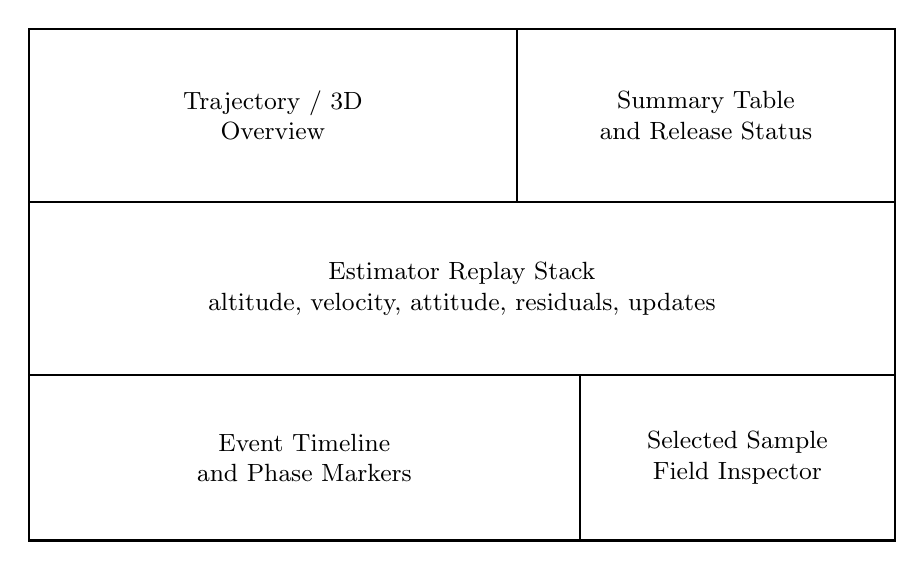
\begin{tikzpicture}[font=\small]
\draw[thick] (0,0) rectangle (11,6.5);
\draw[thick] (0,4.3) -- (11,4.3);
\draw[thick] (0,2.1) -- (11,2.1);
\draw[thick] (6.2,4.3) -- (6.2,6.5);
\draw[thick] (7.0,0) -- (7.0,2.1);
\node[align=center] at (3.1,5.4) {Trajectory / 3D\\Overview};
\node[align=center] at (8.6,5.4) {Summary Table\\and Release Status};
\node[align=center] at (5.5,3.2) {Estimator Replay Stack\\altitude, velocity, attitude, residuals, updates};
\node[align=center] at (3.5,1.05) {Event Timeline\\and Phase Markers};
\node[align=center] at (9.0,1.05) {Selected Sample\\Field Inspector};
\end{tikzpicture}
\end{adjustbox}
\caption{Implementation-informed dashboard layout for the Caelum offline analysis tool, abstracted from the supplied MATLAB dashboard screenshots. The layout emphasizes linked spatial, temporal, event, and summary views.}
\label{fig:dashboard}
\end{figure}

%==============================================================================
\section{TRUTH-AWARE LOGS AND VALIDATION}
%==============================================================================

\subsection{Synthetic Truth-Aware Logs}
\code{generateTruthAwareCaelumLog} and \code{generateTruthAwareCaelumLogV2} provide controlled input data with known truth fields. These generators are essential for separating two questions that are often conflated: whether the estimator behaves correctly and whether a real flight log contains enough information to evaluate that behavior.

\subsection{Vertical Replay Validation}
\code{validate\_vertical\_replay\_stack.m} should verify the complete vertical path: required field presence, import alignment, vertical EKF initialization, prediction, barometric update, output field generation, and dashboard readiness. This test is especially important because vertical performance is one of the most interpretable and safety-relevant views in post-flight review.

\subsection{Release Validation}
\code{validate\_caelum\_release.m} should be treated as the project-level acceptance script. A mature release validation should exercise:
\begin{enumerate}[leftmargin=*,nosep]
\item robust import and schema alignment,
\item log cleaning and attitude-field attachment,
\item vertical and 3D replay paths,
\item event detection and summary-table generation,
\item dashboard and overview plotting without runtime errors,
\item Monte Carlo summary generation, and
\item summary or figure export.
\end{enumerate}

\begin{table*}[t]
\caption{Validation artifacts and the risks they control}
\centering
\begin{tabularx}{\textwidth}{l Y Y}
\toprule
Artifact & Validation purpose & Controlled risk \\
\midrule
\code{run\_caelum\_example.m} & Demonstrates the primary user workflow from log to dashboard & Package appears complete but lacks a runnable entry point \\
\code{validate\_vertical\_replay\_stack.m} & Tests vertical estimator replay and required fields & Broken altitude replay or missing vertical outputs \\
\code{validate\_caelum\_release.m} & Exercises release-level behavior across import, replay, plotting, and export & Regression after package integration changes \\
\code{generateTruthAwareCaelumLog} / \code{V2} & Provides known-truth input for estimator and dashboard checks & Validation depending only on uncertain real logs \\
\code{runMonteCarloValidation} & Evaluates behavior across repeated trials or noise conditions & Single-case success hiding estimator fragility \\
\bottomrule
\end{tabularx}
\label{tab:validation}
\end{table*}

%==============================================================================
\section{REQUIREMENTS-TO-DELIVERABLES TRACEABILITY}
%==============================================================================

\begin{table*}[t]
\caption{Requirements traceability matrix for the Caelum MATLAB analysis project}
\centering
\begin{tabularx}{\textwidth}{l Y Y Y}
\toprule
ID & Requirement & Evidence / artifact & Verification mode \\
\midrule
R1 & The project shall provide a runnable example workflow & \code{run\_caelum\_example.m} & example execution and generated figures \\
R2 & Imported logs shall be mapped to a canonical analysis schema & \code{importLogRobust}, \code{alignImportedSchema} & schema tests and field-contract checks \\
R3 & Firmware SD-card logs shall have a documented MATLAB contract & \code{getFirmwareSdlogSchema} & schema review and import replay \\
R4 & Vertical replay inputs and outputs shall be explicitly contracted & \code{getVerticalReplayFieldContract} & \code{validate\_vertical\_replay\_stack.m} \\
R5 & The analysis shall support vertical EKF replay and barometric updates & \code{runVerticalEKF}, \code{predictVerticalEKF}, \code{updateVerticalEKFBaro} & truth-aware logs and residual checks \\
R6 & The analysis shall support 3D replay with attitude and GPS handling & \code{run3DEKF}, \code{predict3DEKF}, \code{update3DEKFGPS} & synthetic log replay and 3D overview plots \\
R7 & Quaternion-derived quantities shall be normalized and consistently transformed & quaternion utility functions & unit tests on known rotations \\
R8 & Events and summaries shall be generated algorithmically & \code{detectEvents}, \code{summarizeLog}, \code{makeSummaryTable} & expected-event tests and table inspection \\
R9 & Dashboard and figures shall be exportable for review artifacts & \code{plotDashboard}, \code{exportFigures}, \code{exportSummary} & release validation and generated artifacts \\
R10 & Vertical replay diagnostics shall expose measurement gating, covariance, bias, quality, and replay-error behavior & \code{plotDashboard}, vertical replay outputs, quality flags & screenshot review and vertical validation replay \\
R11 & Integrated 3D review shall expose GPS fusion, wind estimates, 3D trajectory, and event timing & \code{plotOverview3D}, \code{plotDashboard}, \code{estimateWind}, GPS update outputs & integrated dashboard review \\
R12 & Release health shall be checkable through a top-level validation script & \code{validate\_caelum\_release.m} & release gate execution \\
\bottomrule
\end{tabularx}
\label{tab:traceability}
\end{table*}

%==============================================================================
\section{DISCUSSION OF ENGINEERING RISKS}
%==============================================================================

\subsection{Schema Drift}
The most likely long-term risk is schema drift between firmware logs, generated synthetic logs, and MATLAB analysis expectations. Caelum mitigates this through explicit schema and field-contract functions, but those contracts must remain part of release validation.

\subsection{Estimator Provenance Ambiguity}
Dashboard users must be able to distinguish raw firmware estimates, MATLAB replay estimates, truth-aware synthetic states, and derived diagnostic fields. If these appear as visually similar traces without provenance, the dashboard can mislead even when the code is numerically correct.

\subsection{Quaternion Convention Errors}
Quaternion ordering, frame convention, and rotation direction errors are subtle and can contaminate gravity compensation, Euler plots, and 3D replay. The project should maintain small deterministic tests for known rotations and gravity-vector transformations.

\subsection{Validation Narrowness}
A dashboard that passes one example log may still fail on real telemetry diversity. This motivates both robust import and Monte Carlo validation, as well as release tests that exercise firmware-style and truth-aware paths.

%==============================================================================
\section{CONCLUSION}
%==============================================================================

Caelum is a MATLAB post-flight offline analysis stack built around replay, schema discipline, estimator reconstruction, event detection, and dashboard visualization. Its engineering value comes from the integration of many small but reviewable components: robust import, schema alignment, cleaning, vertical and 3D EKF replay, quaternion transformations, wind estimation, summary generation, plotting, figure export, firmware compatibility, and validation scripts. The dashboard is therefore not the entire project; it is the visible review surface of a deterministic analysis pipeline. By treating configuration, field contracts, replay outputs, and validation artifacts as first-class engineering products, Caelum provides a rigorous foundation for post-flight diagnosis and release-quality documentation.

%==============================================================================
% APPENDICES
%==============================================================================
\appendix

\section{SUGGESTED MODULE MAP}

\begin{equation*}
\begin{aligned}
&\texttt{scripts/} && \texttt{run\_caelum\_example, validate\_caelum\_release,}\\
& && \texttt{validate\_vertical\_replay\_stack}\\[2pt]
&\texttt{+caelum/import} && \texttt{importLog, importLogRobust,}\\
& && \texttt{alignImportedSchema, getFirmwareSdlogSchema}\\[2pt]
&\texttt{+caelum/replay} && \texttt{runVerticalEKF, run3DEKF, replayEstimator,}\\
& && \texttt{runFirmwareVerticalEstimator}\\[2pt]
&\texttt{+caelum/attitude} && \texttt{normalizeQuaternion, propagateQuaternion,}\\
& && \texttt{quaternionToRotationMatrix, quaternionToEulerZYX}\\[2pt]
&\texttt{+caelum/analysis} && \texttt{analyzeLog, detectEvents, estimateWind,}\\
& && \texttt{summarizeLog, makeSummaryTable}\\[2pt]
&\texttt{+caelum/plots} && \texttt{plotDashboard, plotOverview, plotOverview3D,}\\
& && \texttt{plotMonteCarloSummary, exportFigures}
\end{aligned}
\end{equation*}

\section{FIGURE PREPARATION NOTE}

For publication artifacts, dashboard figures should be exported from MATLAB at fixed resolution using \code{exportFigures} or an equivalent scripted export path. Desktop screenshots are useful for design discussion, but scripted exports are preferable for final PDF generation because they remove operating-system chrome, preserve repeatable sizing, and keep the manuscript build independent of absolute desktop paths.

\section{POST-FLIGHT REVIEW CHECKLIST}

\begin{enumerate}[leftmargin=*,nosep]
\item Confirm that the log imports through \code{importLogRobust}.
\item Confirm that \code{alignImportedSchema} maps the log to the canonical field set.
\item Run \code{cleanLog} and inspect rejected, repaired, or missing samples.
\item Verify that attitude fields are present or attached through \code{attachPhase1AttitudeFields}.
\item Run vertical replay and inspect altitude, velocity, covariance, and barometric residuals.
\item Run 3D replay when GPS and attitude fields are available.
\item Inspect \code{detectEvents} output before interpreting the dashboard narrative.
\item Generate \code{plotDashboard}, \code{plotOverview}, and \code{plotOverview3D} as applicable.
\item Export the summary table and figures for the engineering record.
\item Run release validation before treating the output as a stable package result.
\end{enumerate}

\section*{REFERENCES}
\begin{thebibliography}{99}

\bibitem{caelum_release}
Richardson, D., \emph{Caelum Phase 1 Fully Integrated MATLAB Release Notes}, project release artifact, 2026.

\bibitem{caelum_code}
Richardson, D., \emph{Caelum MATLAB Package Source}, \code{+caelum} namespace containing post-flight import, replay, analysis, and plotting functions.

\bibitem{matlab_timetable}
MathWorks, \emph{timetable: Tables for time series data, with timestamped rows and variables of different types}. Available: \url{https://www.mathworks.com/help/matlab/ref/timetable.html}.

\bibitem{welch}
Welch, G., and Bishop, G., 2006, \emph{An Introduction to the Kalman Filter}, University of North Carolina at Chapel Hill.

\bibitem{titterton}
Titterton, D., and Weston, J. L., 2004, \emph{Strapdown Inertial Navigation Technology}, 2nd ed., Institution of Electrical Engineers, London.

\bibitem{kuipers}
Kuipers, J. B., 1999, \emph{Quaternions and Rotation Sequences}, Princeton University Press, Princeton, NJ.

\end{thebibliography}

\end{document}
